% Options for packages loaded elsewhere
\PassOptionsToPackage{unicode}{hyperref}
\PassOptionsToPackage{hyphens}{url}
%
\documentclass[
  english,
  man,floatsintext]{apa6}
\usepackage{lmodern}
\usepackage{amssymb,amsmath}
\usepackage{ifxetex,ifluatex}
\ifnum 0\ifxetex 1\fi\ifluatex 1\fi=0 % if pdftex
  \usepackage[T1]{fontenc}
  \usepackage[utf8]{inputenc}
  \usepackage{textcomp} % provide euro and other symbols
\else % if luatex or xetex
  \usepackage{unicode-math}
  \defaultfontfeatures{Scale=MatchLowercase}
  \defaultfontfeatures[\rmfamily]{Ligatures=TeX,Scale=1}
\fi
% Use upquote if available, for straight quotes in verbatim environments
\IfFileExists{upquote.sty}{\usepackage{upquote}}{}
\IfFileExists{microtype.sty}{% use microtype if available
  \usepackage[]{microtype}
  \UseMicrotypeSet[protrusion]{basicmath} % disable protrusion for tt fonts
}{}
\makeatletter
\@ifundefined{KOMAClassName}{% if non-KOMA class
  \IfFileExists{parskip.sty}{%
    \usepackage{parskip}
  }{% else
    \setlength{\parindent}{0pt}
    \setlength{\parskip}{6pt plus 2pt minus 1pt}}
}{% if KOMA class
  \KOMAoptions{parskip=half}}
\makeatother
\usepackage{xcolor}
\IfFileExists{xurl.sty}{\usepackage{xurl}}{} % add URL line breaks if available
\IfFileExists{bookmark.sty}{\usepackage{bookmark}}{\usepackage{hyperref}}
\hypersetup{
  pdftitle={Re-analysing the data from Moffatt et al. (2020): A textbook illustration of the absence of evidence fallacy},
  pdflang={en-EN},
  pdfkeywords={NHST, Bayesian, fallacy, reanalysis, inner speech, rumination, electromyography},
  hidelinks,
  pdfcreator={LaTeX via pandoc}}
\urlstyle{same} % disable monospaced font for URLs
\usepackage{color}
\usepackage{fancyvrb}
\newcommand{\VerbBar}{|}
\newcommand{\VERB}{\Verb[commandchars=\\\{\}]}
\DefineVerbatimEnvironment{Highlighting}{Verbatim}{commandchars=\\\{\}}
% Add ',fontsize=\small' for more characters per line
\usepackage{framed}
\definecolor{shadecolor}{RGB}{248,248,248}
\newenvironment{Shaded}{\begin{snugshade}}{\end{snugshade}}
\newcommand{\AlertTok}[1]{\textcolor[rgb]{0.94,0.16,0.16}{#1}}
\newcommand{\AnnotationTok}[1]{\textcolor[rgb]{0.56,0.35,0.01}{\textbf{\textit{#1}}}}
\newcommand{\AttributeTok}[1]{\textcolor[rgb]{0.77,0.63,0.00}{#1}}
\newcommand{\BaseNTok}[1]{\textcolor[rgb]{0.00,0.00,0.81}{#1}}
\newcommand{\BuiltInTok}[1]{#1}
\newcommand{\CharTok}[1]{\textcolor[rgb]{0.31,0.60,0.02}{#1}}
\newcommand{\CommentTok}[1]{\textcolor[rgb]{0.56,0.35,0.01}{\textit{#1}}}
\newcommand{\CommentVarTok}[1]{\textcolor[rgb]{0.56,0.35,0.01}{\textbf{\textit{#1}}}}
\newcommand{\ConstantTok}[1]{\textcolor[rgb]{0.00,0.00,0.00}{#1}}
\newcommand{\ControlFlowTok}[1]{\textcolor[rgb]{0.13,0.29,0.53}{\textbf{#1}}}
\newcommand{\DataTypeTok}[1]{\textcolor[rgb]{0.13,0.29,0.53}{#1}}
\newcommand{\DecValTok}[1]{\textcolor[rgb]{0.00,0.00,0.81}{#1}}
\newcommand{\DocumentationTok}[1]{\textcolor[rgb]{0.56,0.35,0.01}{\textbf{\textit{#1}}}}
\newcommand{\ErrorTok}[1]{\textcolor[rgb]{0.64,0.00,0.00}{\textbf{#1}}}
\newcommand{\ExtensionTok}[1]{#1}
\newcommand{\FloatTok}[1]{\textcolor[rgb]{0.00,0.00,0.81}{#1}}
\newcommand{\FunctionTok}[1]{\textcolor[rgb]{0.00,0.00,0.00}{#1}}
\newcommand{\ImportTok}[1]{#1}
\newcommand{\InformationTok}[1]{\textcolor[rgb]{0.56,0.35,0.01}{\textbf{\textit{#1}}}}
\newcommand{\KeywordTok}[1]{\textcolor[rgb]{0.13,0.29,0.53}{\textbf{#1}}}
\newcommand{\NormalTok}[1]{#1}
\newcommand{\OperatorTok}[1]{\textcolor[rgb]{0.81,0.36,0.00}{\textbf{#1}}}
\newcommand{\OtherTok}[1]{\textcolor[rgb]{0.56,0.35,0.01}{#1}}
\newcommand{\PreprocessorTok}[1]{\textcolor[rgb]{0.56,0.35,0.01}{\textit{#1}}}
\newcommand{\RegionMarkerTok}[1]{#1}
\newcommand{\SpecialCharTok}[1]{\textcolor[rgb]{0.00,0.00,0.00}{#1}}
\newcommand{\SpecialStringTok}[1]{\textcolor[rgb]{0.31,0.60,0.02}{#1}}
\newcommand{\StringTok}[1]{\textcolor[rgb]{0.31,0.60,0.02}{#1}}
\newcommand{\VariableTok}[1]{\textcolor[rgb]{0.00,0.00,0.00}{#1}}
\newcommand{\VerbatimStringTok}[1]{\textcolor[rgb]{0.31,0.60,0.02}{#1}}
\newcommand{\WarningTok}[1]{\textcolor[rgb]{0.56,0.35,0.01}{\textbf{\textit{#1}}}}
\usepackage{graphicx}
\makeatletter
\def\maxwidth{\ifdim\Gin@nat@width>\linewidth\linewidth\else\Gin@nat@width\fi}
\def\maxheight{\ifdim\Gin@nat@height>\textheight\textheight\else\Gin@nat@height\fi}
\makeatother
% Scale images if necessary, so that they will not overflow the page
% margins by default, and it is still possible to overwrite the defaults
% using explicit options in \includegraphics[width, height, ...]{}
\setkeys{Gin}{width=\maxwidth,height=\maxheight,keepaspectratio}
% Set default figure placement to htbp
\makeatletter
\def\fps@figure{htbp}
\makeatother
\setlength{\emergencystretch}{3em} % prevent overfull lines
\providecommand{\tightlist}{%
  \setlength{\itemsep}{0pt}\setlength{\parskip}{0pt}}
\setcounter{secnumdepth}{-\maxdimen} % remove section numbering
% Make \paragraph and \subparagraph free-standing
\ifx\paragraph\undefined\else
  \let\oldparagraph\paragraph
  \renewcommand{\paragraph}[1]{\oldparagraph{#1}\mbox{}}
\fi
\ifx\subparagraph\undefined\else
  \let\oldsubparagraph\subparagraph
  \renewcommand{\subparagraph}[1]{\oldsubparagraph{#1}\mbox{}}
\fi
% Manuscript styling
\usepackage{upgreek}
\captionsetup{font=singlespacing,justification=justified}

% Table formatting
\usepackage{longtable}
\usepackage{lscape}
% \usepackage[counterclockwise]{rotating}   % Landscape page setup for large tables
\usepackage{multirow}		% Table styling
\usepackage{tabularx}		% Control Column width
\usepackage[flushleft]{threeparttable}	% Allows for three part tables with a specified notes section
\usepackage{threeparttablex}            % Lets threeparttable work with longtable

% Create new environments so endfloat can handle them
% \newenvironment{ltable}
%   {\begin{landscape}\begin{center}\begin{threeparttable}}
%   {\end{threeparttable}\end{center}\end{landscape}}
\newenvironment{lltable}{\begin{landscape}\begin{center}\begin{ThreePartTable}}{\end{ThreePartTable}\end{center}\end{landscape}}

% Enables adjusting longtable caption width to table width
% Solution found at http://golatex.de/longtable-mit-caption-so-breit-wie-die-tabelle-t15767.html
\makeatletter
\newcommand\LastLTentrywidth{1em}
\newlength\longtablewidth
\setlength{\longtablewidth}{1in}
\newcommand{\getlongtablewidth}{\begingroup \ifcsname LT@\roman{LT@tables}\endcsname \global\longtablewidth=0pt \renewcommand{\LT@entry}[2]{\global\advance\longtablewidth by ##2\relax\gdef\LastLTentrywidth{##2}}\@nameuse{LT@\roman{LT@tables}} \fi \endgroup}

% \setlength{\parindent}{0.5in}
% \setlength{\parskip}{0pt plus 0pt minus 0pt}

% \usepackage{etoolbox}
\makeatletter
\patchcmd{\HyOrg@maketitle}
  {\section{\normalfont\normalsize\abstractname}}
  {\section*{\normalfont\normalsize\abstractname}}
  {}{\typeout{Failed to patch abstract.}}
\makeatother
\shorttitle{The absence of evidence fallacy}
\author{Ladislas Nalborczyk\textsuperscript{1}}
\affiliation{
\vspace{0.5cm}
\textsuperscript{1} Univ. Grenoble Alpes, CNRS, Grenoble INP, GIPSA-lab, 38000 Grenoble, France}
\authornote{

Correspondence concerning this article should be addressed to Ladislas Nalborczyk, GIPSA-lab, CNRS, Univ. Grenoble Alpes, 11 Rue des Mathématiques, 38400 Saint-Martin-d'Hères, France. E-mail: ladislas.nalborczyk@gipsa-lab.fr}
\keywords{NHST, Bayesian, fallacy, reanalysis, inner speech, rumination, electromyography}
\usepackage{lineno}

\linenumbers
\usepackage{csquotes}
\ifxetex
  % Load polyglossia as late as possible: uses bidi with RTL langages (e.g. Hebrew, Arabic)
  \usepackage{polyglossia}
  \setmainlanguage[]{english}
\else
  \usepackage[shorthands=off,main=english]{babel}
\fi
\newlength{\cslhangindent}
\setlength{\cslhangindent}{1.5em}
\newenvironment{cslreferences}%
  {\setlength{\parindent}{0pt}%
  \everypar{\setlength{\hangindent}{\cslhangindent}}\ignorespaces}%
  {\par}

\title{Re-analysing the data from Moffatt et al. (\protect\hyperlink{ref-moffatt_inner_2020}{2020}): A textbook illustration of the absence of evidence fallacy}

\date{}

\abstract{
Moffatt et al. (\protect\hyperlink{ref-moffatt_inner_2020}{2020}) reported the results of an experiment (N = 26 in the final sample) comparing the facial (surface) electromyographic correlates of mental rumination and distraction, following an experimentally induced stressor. Based on the absence of significant difference in the perioral muscular activity between the rumination and distraction conditions, Moffatt et al. (\protect\hyperlink{ref-moffatt_inner_2020}{2020}) concluded that (the \emph{self-reported}) inner experience was unrelated to peripheral muscular activity as assessed using surface electromyography. We suggest this conclusion is hasty and based on waggly evidence. Indeed, concluding on the absence of an effect based on a low-powered statistical test is strongly problematic/uninformative. Moreover, the relation between self-reports and physiological measures was not \emph{directly} assessed, but only indirectly inferred from differences (or absence thereof) in group means. Given the ample inter-individual variability in these measures (as suggested through our reanalysis), we think inferring the individual-level relation between self-reports and physiological measures from group means is inappropriate. Given these limitations, we conclude that it is unclear whether the target article adds to the current/extent knowledge and we suggest ways forward, both from a theoretical and from a methodological perspective. Complete source code, reproducible analyses, and figures are available at \url{https://github.com/lnalborczyk/inner_experience_EMG}.
}

\begin{document}
\maketitle

Wordcount (excluding abstract, references, tables, and figures): 1527

\newpage

\hypertarget{introduction}{%
\section{Introduction}\label{introduction}}

The activity of silently talking to oneself or ``inner speech'' is a foundational ability\ldots{} despite its multiple adaptive functions in everyday life, inner speech can go awry and leads to sustained negative\ldots{} These inner speech ``dysfunctions'' (for reviews, see Alderson-Day \& Fernyhough, \protect\hyperlink{ref-alderson-day_inner_2015}{2015}; Lœvenbruck et al., \protect\hyperlink{ref-loevenbruck_cognitive_2018}{2018}; Perrone-Bertolotti et al., \protect\hyperlink{ref-perrone-bertolotti_what_2014}{2014})\ldots{}

Given the predominantly verbal nature of rumination {[}{]}, we previously proposed to study rumination as other forms of inner speech have been studied in the past, namely using surface electromyography and motor interference protocols (e.g., Nalborczyk et al., \protect\hyperlink{ref-nalborczyk_orofacial_2017}{2017}; Nalborczyk, \protect\hyperlink{ref-nalborczyk_understanding_2019}{2019}; Nalborczyk, Perrone-Bertolotti, et al., \protect\hyperlink{ref-nalborczyk_articulatory_2020}{2020}; Nalborczyk, Grandchamp, et al., \protect\hyperlink{ref-nalborczyk_can_2020}{2020})\ldots{}

Moffatt et al. (\protect\hyperlink{ref-moffatt_inner_2020}{2020}), Grandchamp et al. (\protect\hyperlink{ref-grandchamp_condialint_2019}{2019}), Wilkinson and Fernyhough (\protect\hyperlink{ref-wilkinson_auditory_2017}{2017}), Nalborczyk, Batailler, et al. (\protect\hyperlink{ref-nalborczyk_introduction_2019}{2019})\ldots{}

The main conclusion from Moffatt et al. (\protect\hyperlink{ref-moffatt_inner_2020}{2020}) is that inner experience between induced rumination and distraction differs ``without a change in electromyographic correlates of inner speech''. In other words, their conclusion is that inner experience is unrelated (or loosely related) to the electromyographic correlates of inner speech, which are thought to be represented mostly by the EMG amplitude recorded over the OOI and OOS muscles. However, for this in-sample observation to be of interest in an out-of-sample context (i.e., to be informative of other non-observed individuals, or said otherwise, to brings information about the population), this absence of difference has to be based on sufficiently powered sample size (given the target effect size) and on reliable measures\ldots{} Moreover, a simple visual exploration of the data reveals important variability between individuals in the main effect of interest. That is, some participants had higher perioral (OOS and OOI) muscular activity in the rumination condition than in the distraction condition, and some other participants showed the reverse pattern. This suggests unexplored variation in the determinants of this effects (e.g., the content of the inner experience). Indeed, the relation between the inner experience and the physiological correlates of inner speech production was only inferred from group means. However, given the previous point, this appears highly problematic. We explore each of these limitations and suggests ways forward in the following section.

\hypertarget{exploring-the-data}{%
\section{Exploring the data}\label{exploring-the-data}}

\begin{figure}[!htb]

{\centering 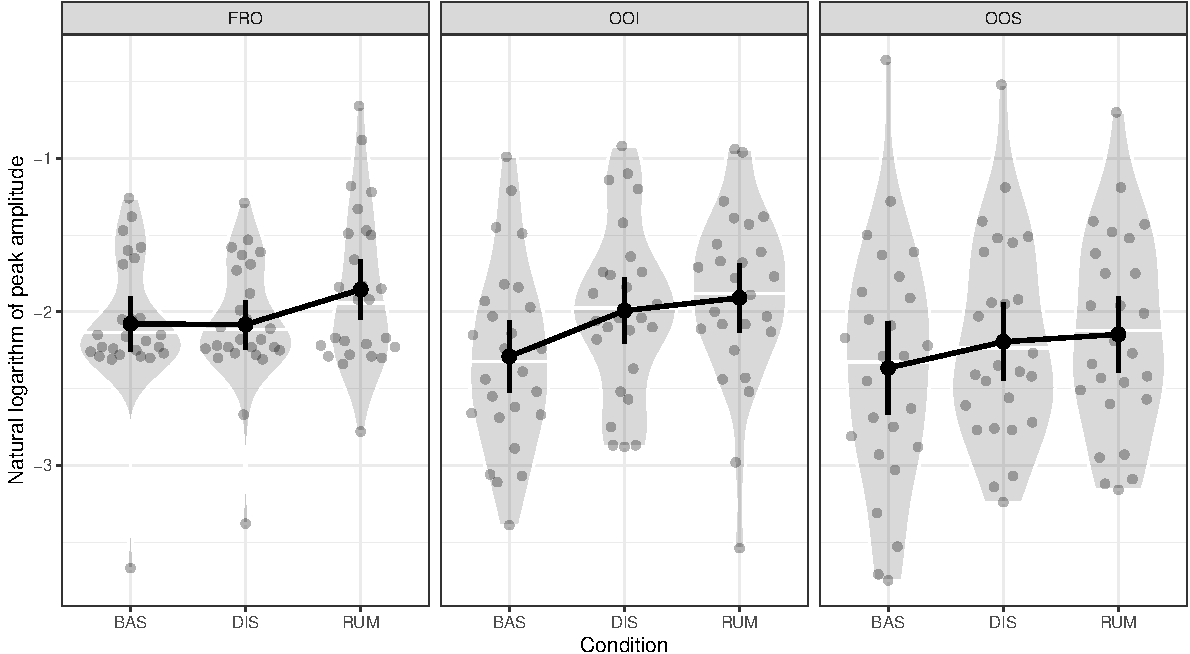
\includegraphics[width=1\linewidth]{reanalysis_files/figure-latex/general-1} 

}

\caption{Average log-EMG amplitude by muscle and condition. The black dots and intervals represent the by-group average and 95\% confidence interval (N = 26). The horizontal white line in the violin plot represents the median. The grey dots represent the individual-level average natural logarithm of the EMG amplitude by muscle and condition.}\label{fig:general}
\end{figure}

\ldots{}

\hypertarget{concluding-on-the-null-from-low-powered-studies}{%
\subsection{Concluding on the null from low-powered studies}\label{concluding-on-the-null-from-low-powered-studies}}

There is an infamous tradition of running uninformative null-hypothesis significance tests in Psychology (e.g., Meehl, \protect\hyperlink{ref-harlow_problem_1997}{1997}, \protect\hyperlink{ref-meehl_theoretical_1978}{1978}, \protect\hyperlink{ref-meehl_why_1990}{1990}\protect\hyperlink{ref-meehl_why_1990}{a}, \protect\hyperlink{ref-meehl_appraising_1990-1}{1990}\protect\hyperlink{ref-meehl_appraising_1990-1}{b}, \protect\hyperlink{ref-meehl_theory-testing_1967}{1967}). By ``uninformative'', we mean that some null-hypothesis significance tests are often \emph{not} diagnostic with regards to the substantive question of interest\ldots{}

As highlighted by many authors (e.g., {\textbf{???}}), concluding on an absence of difference based on not obtaining evidence for the difference is the continuous extension of the logical fallacy of the\ldots{} The argument from ignorance, such as ``Science has found no proof of intelligent life nearby us in space, therefore intelligent life does not exist nearby us in space.''\ldots{} the absence of evidence fallacy or fallacy of acceptance\ldots{}

This problem is tackled in modern usages of null-hypothesis significance test by ensuring that the test has good \emph{severity} (e.g., Mayo \& Spanos, \protect\hyperlink{ref-mayo_severe_2006}{2006}; Mayo, \protect\hyperlink{ref-mayo_statistical_2018}{2018}). In general terms, we have evidence for a claim to the extent that it survives a stringent scrutiny, that is if it survives \emph{severe tests}. In other words, some claim (e.g., \(\theta = 0\)) is said to be \emph{severely tested}) if it had great chances of being falsified, was the claim false. More formally, we can define \(\text{SEV}(T, x0, H)\), the severity with which claim \(H\) passes test \(T\) with outcome \(x0\), and \(\text{SEV}(\mu > \mu_{1}) = \Pr(d(X) \leq d(x0); \mu = \mu_{1})\) (Mayo, \protect\hyperlink{ref-mayo_statistical_2018}{2018}; Mayo \& Spanos, \protect\hyperlink{ref-mayo_severe_2006}{2006})\ldots To put it simply\ldots{} \url{https://www.analytics-toolkit.com/glossary/severity/}\ldots{}

Anticipating the critics on the power of their study (a critic that was probably raised during peer review), Moffatt et al. (\protect\hyperlink{ref-moffatt_inner_2020}{2020}) report the results of a (possibly ran a posteriori) power analysis using the effect size reported in Nalborczyk et al. (\protect\hyperlink{ref-nalborczyk_orofacial_2017}{2017}) of \(d = 0.72\), which is highly optimistic estimate of the substantive effect of interest in the target article (i.e., the difference in EMG amplitude between the rumination and distraction conditions) as this effects represents the standardised mean difference \emph{between a rest period and a rumination one} (Nalborczyk et al., \protect\hyperlink{ref-nalborczyk_orofacial_2017}{2017})\ldots{}

\begin{Shaded}
\begin{Highlighting}[]
\CommentTok{\# How many participants do we need for a target statistical power of 0.8?}
\KeywordTok{library}\NormalTok{(pwr)}
\KeywordTok{pwr.t.test}\NormalTok{(}
  \DataTypeTok{d =} \FloatTok{0.72}\NormalTok{, }\DataTypeTok{sig.level =} \FloatTok{0.05}\NormalTok{, }\DataTypeTok{power =} \FloatTok{0.8}\NormalTok{,}
  \DataTypeTok{type =} \StringTok{"one.sample"}\NormalTok{, }\DataTypeTok{alternative =} \StringTok{"two.sided"}
\NormalTok{  )}
\end{Highlighting}
\end{Shaded}

\begin{verbatim}
## 
##      One-sample t test power calculation 
## 
##               n = 17.16004
##               d = 0.72
##       sig.level = 0.05
##           power = 0.8
##     alternative = two.sided
\end{verbatim}

We suggest the (a priori) power of the study ran by Moffatt et al. (\protect\hyperlink{ref-moffatt_inner_2020}{2020}) was was much lower than suggested by the authors. Indeed, we may speculate that the effect (i.e., the standardised mean difference in EMG amplitude) between the rumination and distraction condition may be much weaker than the effect (i.e., the standardised mean difference in EMG amplitude) between the rumination and the rest conditions. If we assume that the former is half the size of the latter (which seems reasonable given the distribution of effects sizes in Experimental Psychology, e.g., Szucs \& Ioannidis, \protect\hyperlink{ref-szucs_empirical_2017}{2017}), therefore the a priori power of the main statistical test from Moffatt et al. (\protect\hyperlink{ref-moffatt_inner_2020}{2020}) is around \(0.44\), meaning that they had less than 1 chance over two to find a significant effect, given the effect in the population is actually \(0.36\). Because this is less than the chance of obtaining a head in a coin flip, we feel these resources may have been better invested.

\begin{Shaded}
\begin{Highlighting}[]
\CommentTok{\# A priori power for n = 26 (per condition) and d = 0.36}
\KeywordTok{pwr.t.test}\NormalTok{(}
  \DataTypeTok{n =} \DecValTok{26}\NormalTok{, }\DataTypeTok{d =} \FloatTok{0.72} \OperatorTok{/}\StringTok{ }\DecValTok{2}\NormalTok{, }\DataTypeTok{sig.level =} \FloatTok{0.05}\NormalTok{,}
  \DataTypeTok{type =} \StringTok{"one.sample"}\NormalTok{, }\DataTypeTok{alternative =} \StringTok{"two.sided"}
\NormalTok{  )}
\end{Highlighting}
\end{Shaded}

\begin{verbatim}
## 
##      One-sample t test power calculation 
## 
##               n = 26
##               d = 0.36
##       sig.level = 0.05
##           power = 0.4228455
##     alternative = two.sided
\end{verbatim}

Anticipating again the legitimate critique that the absence of a significant difference is not \emph{necessarily} ``significant'' evidence of the absence of the effect, Moffatt et al. (\protect\hyperlink{ref-moffatt_inner_2020}{2020}) report the following Bayes factor analysis:

\begin{quote}
``{[}\ldots{]} therefore it is possible that the sample size of the present study lacked sufficient power to detect the effect of rumination on muscle activity. In order to test this, a Bayesian paired samples t-test was conducted for the peak log values of muscle activity between the rumination and distraction conditions. This revealed strong evidence in favour of the alternative hypothesis for the FRO muscle (\(B_{10} = 18.79\)), and moderate evidence in favour of the null hypothesis for the OOS (\(B_{10} = 0.232\)) and OOI (\(B_{10} = 0.278\)) muscles, according to current guidelines for interpreting Bayes factors {[}43{]}.''
\end{quote}

While we appreciate the effort, the current approach poses new problems. First, contrary to what the authors suggest, computing a BF (i.e., comparing two models) does not solve at all the problem of low power. Second, no details are given with regards to the exact models that were compared. Second\ldots{} Third, and most importantly, the BFs indicate moderate evidence in favour of the null for the OOI and OOS muscles. More precisely, these BFs indicated that the (observed) data are \(1 / 0.232 \approx 4.31\) times more likely under the null than under the alternative hypothesis for the OOS and \(1 / 0.278 \approx 3.6\) times more likely under the null than under the alternative hypothesis for the OOI. In other words, the evidence is favour of the null is relatively weak and sensitivity analyses (i.e., reporting the BF with different prior scales) may unsurprisingly results in various BFs\ldots{} For instance\ldots{} Finally and most importantly, the power\ldots{}

\begin{Shaded}
\begin{Highlighting}[]
\KeywordTok{library}\NormalTok{(BayesFactor)}
\KeywordTok{ttestBF}\NormalTok{(}\DataTypeTok{x =}\NormalTok{ df2}\OperatorTok{$}\NormalTok{OOI[df2}\OperatorTok{$}\NormalTok{condition }\OperatorTok{==}\StringTok{ "RUM"}\NormalTok{], }\DataTypeTok{y =}\NormalTok{ df2}\OperatorTok{$}\NormalTok{OOI[df2}\OperatorTok{$}\NormalTok{condition }\OperatorTok{==}\StringTok{ "DIS"}\NormalTok{], }\DataTypeTok{paired =} \OtherTok{TRUE}\NormalTok{, }\DataTypeTok{rscale =} \StringTok{"medium"}\NormalTok{)}
\end{Highlighting}
\end{Shaded}

\begin{verbatim}
## Bayes factor analysis
## --------------
## [1] Alt., r=0.707 : 0.2796158 ±0.03%
## 
## Against denominator:
##   Null, mu = 0 
## ---
## Bayes factor type: BFoneSample, JZS
\end{verbatim}

\begin{Shaded}
\begin{Highlighting}[]
\KeywordTok{ttestBF}\NormalTok{(}\DataTypeTok{x =}\NormalTok{ df2}\OperatorTok{$}\NormalTok{OOI[df2}\OperatorTok{$}\NormalTok{condition }\OperatorTok{==}\StringTok{ "RUM"}\NormalTok{], }\DataTypeTok{y =}\NormalTok{ df2}\OperatorTok{$}\NormalTok{OOI[df2}\OperatorTok{$}\NormalTok{condition }\OperatorTok{==}\StringTok{ "DIS"}\NormalTok{], }\DataTypeTok{paired =} \OtherTok{TRUE}\NormalTok{, }\DataTypeTok{rscale =} \StringTok{"wide"}\NormalTok{)}
\end{Highlighting}
\end{Shaded}

\begin{verbatim}
## Bayes factor analysis
## --------------
## [1] Alt., r=1 : 0.2072665 ±0.06%
## 
## Against denominator:
##   Null, mu = 0 
## ---
## Bayes factor type: BFoneSample, JZS
\end{verbatim}

\begin{Shaded}
\begin{Highlighting}[]
\KeywordTok{ttestBF}\NormalTok{(}\DataTypeTok{x =}\NormalTok{ df2}\OperatorTok{$}\NormalTok{OOI[df2}\OperatorTok{$}\NormalTok{condition }\OperatorTok{==}\StringTok{ "RUM"}\NormalTok{], }\DataTypeTok{y =}\NormalTok{ df2}\OperatorTok{$}\NormalTok{OOI[df2}\OperatorTok{$}\NormalTok{condition }\OperatorTok{==}\StringTok{ "DIS"}\NormalTok{], }\DataTypeTok{paired =} \OtherTok{TRUE}\NormalTok{, }\DataTypeTok{rscale =} \StringTok{"ultrawide"}\NormalTok{)}
\end{Highlighting}
\end{Shaded}

\begin{verbatim}
## Bayes factor analysis
## --------------
## [1] Alt., r=1.414 : 0.1505836 ±0%
## 
## Against denominator:
##   Null, mu = 0 
## ---
## Bayes factor type: BFoneSample, JZS
\end{verbatim}

\begin{Shaded}
\begin{Highlighting}[]
\CommentTok{\# ttestBF(x = df2$OOI[df2$condition == "RUM"], y = df2$OOI[df2$condition == "DIS"], paired = TRUE, rscale = sqrt(2)/2)}
\CommentTok{\# ttestBF(x = df2$OOI[df2$condition == "RUM"], y = df2$OOI[df2$condition == "DIS"], paired = TRUE, rscale = 1)}
\CommentTok{\# ttestBF(x = df2$OOI[df2$condition == "RUM"], y = df2$OOI[df2$condition == "DIS"], paired = TRUE, rscale = sqrt(2) )}
\end{Highlighting}
\end{Shaded}

We fitted a multivariate Bayesian regression model on these data\ldots{} then we generated new datasets from the posterior predictive distribution\ldots{} and computed the Bayes factor in favour of the alternative hypothesis (\(BF_{10}\)) for varying sample sizes from 20 to 200 participants (by increments of 10 participants) with \(10\) simulations (i.e., 1000 simulated datasets) for each sample size\ldots{}

\begin{figure}[!htb]

{\centering 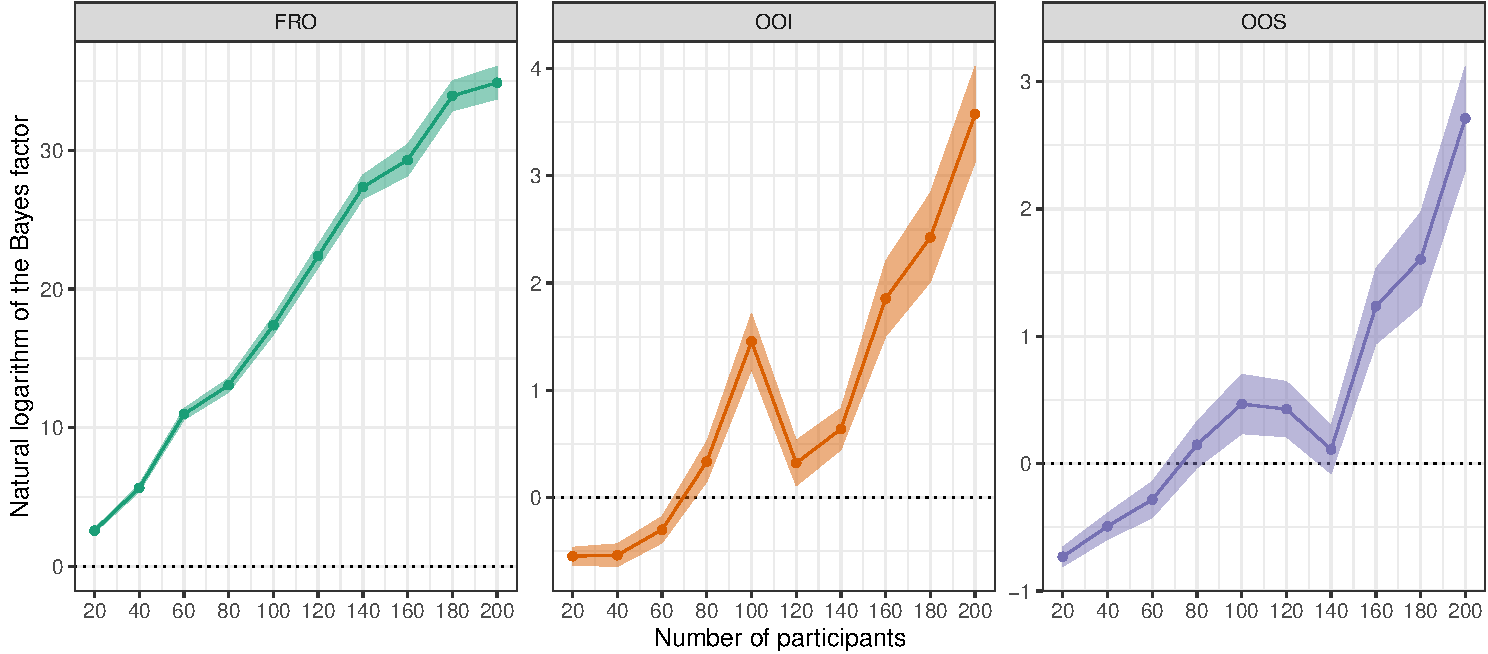
\includegraphics[width=1\linewidth]{reanalysis_files/figure-latex/simulated-power-1} 

}

\caption{Average natural logarithm of the Bayes factor in favour of the alternative hypothesis (BF10), along with its standard error, computed over 1000 datasets of increasing size simulated from the posterior predictive distribution of the varying-intercept multivariate Bayesian regresion model.}\label{fig:simulated-power}
\end{figure}

As shown in Figure \ref{fig:simulated-power}, the BF in favour of the alternative hypothesis is growing proportionally with the sample size\ldots{}

We should keep in mind the limitations of this analysis, which uses simulated datasets form the posterior distribution estimated from\ldots{} which corresponds more or less to the Bayesian analogue of the post-hoc frequentist power analysis, which has been much criticised (e.g., Lakens, \protect\hyperlink{ref-lakens_20_2014}{2014}). However, the present analysis differs from this kind of analysis by relying on the posterior distribution\ldots{} and because we do not aim to reach a dichotomic (e.g., accept/reject) goal but rather to see how the BF amplitude evolves with varying sample sizes.

\hypertarget{manipulating-rumination-within-subject}{%
\subsection{Manipulating rumination within-subject}\label{manipulating-rumination-within-subject}}

In Nalborczyk, Banjac, et al. (\protect\hyperlink{ref-nalborczyk_dissociating_2020}{2020}), we manipulated the modality of rumination (whether it is verbal or non-verbal) in a between-subject manner to avoid order effects\ldots{} In contrast to this approach, Moffatt et al. (\protect\hyperlink{ref-moffatt_inner_2020}{2020}) asked participants to ruminate and then distract themselves (or reciprocally), after an induced stressor (an induced failure)\ldots{}

\begin{figure}[!htb]

{\centering 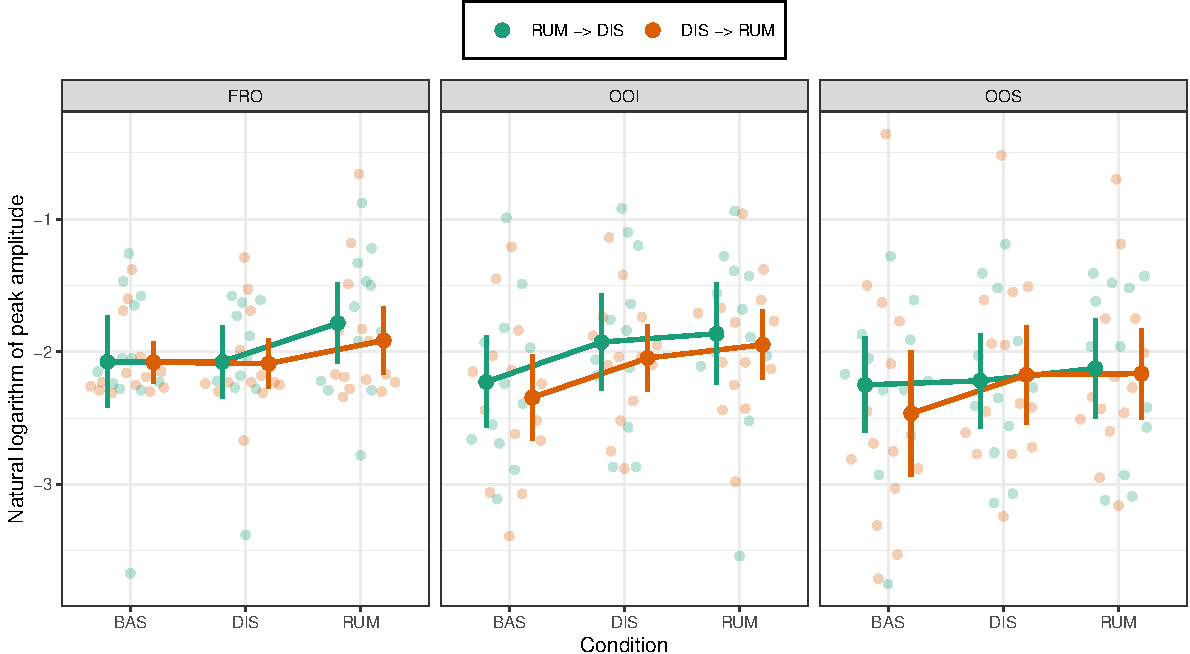
\includegraphics[width=1\linewidth]{reanalysis_files/figure-latex/order-1} 

}

\caption{Average log-EMG amplitude by muscle and condition. The black dots and intervals represent the by-group average and 95\% confidence interval (N = 26). The horizontal white line in the violin plot represents the median. The grey dots represent the individual-level average natural logarithm of the EMG amplitude by muscle and condition.}\label{fig:order}
\end{figure}

About the order effects, Moffatt et al. (\protect\hyperlink{ref-moffatt_inner_2020}{2020}) say:

\begin{quote}
``Unless otherwise reported, the inclusion of order in which the conditions were completed as a between-subjects variable as part of a mixed-design ANOVA produced no significant main effects or interactions involving order.''
\end{quote}

Unfortunately, the same line of reasoning applies for testing the effect of the order, which is even less powered than the test of the main effect of interest, rendering it practically uninformative\ldots{}

\hypertarget{does-everyone}{%
\subsection{Does everyone?}\label{does-everyone}}

Haaf and Rouder (\protect\hyperlink{ref-haaf_developing_2017}{2017})\ldots{}

\begin{figure}[!htb]

{\centering 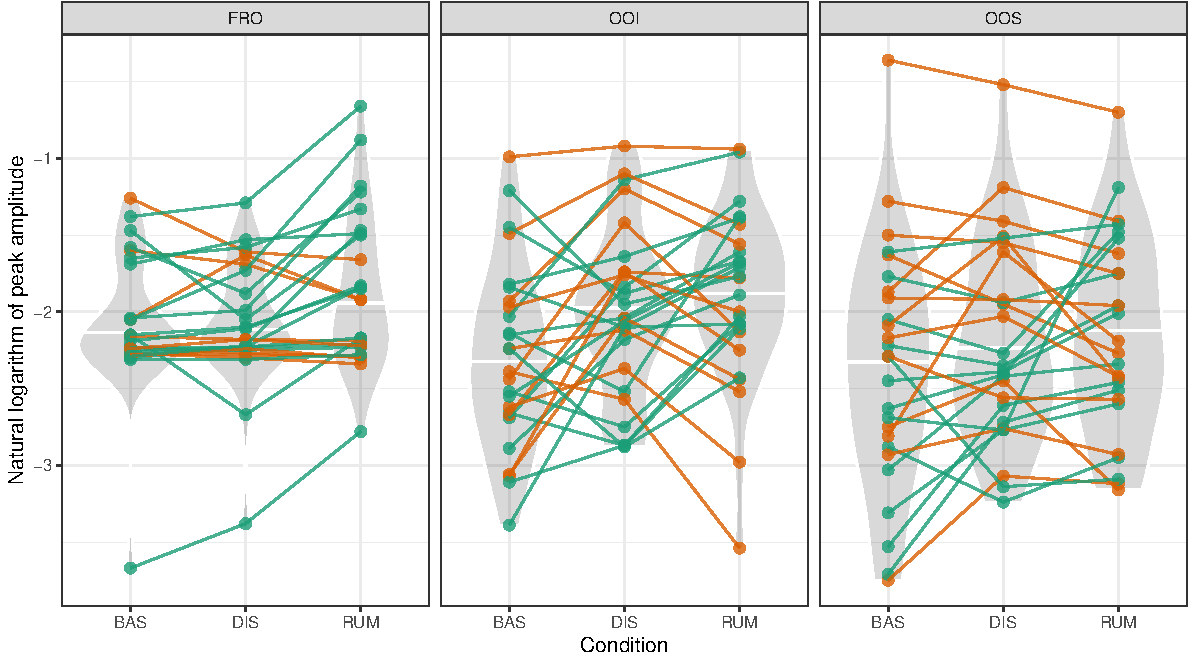
\includegraphics[width=1\linewidth]{reanalysis_files/figure-latex/everyone-1} 

}

\caption{Inter-individual variability in the main effect of interest (i.e., the difference between the rumination and distraction conditions). Green dots and lines represent the average natural logarithm of the EMG amplitude of participants that showed a higher EMG amplitude in the rumination condition than in the distraction condition, whereas orange dots and lines represent the average natural logarithm of the EMG amplitude of participants that showed a higher EMG amplitude in the distraction condition than in the rumination condition.}\label{fig:everyone}
\end{figure}

Huge inter-individual variability\ldots{} which leads to the next point, what is the relation between self-reports and EMG?

\hypertarget{relation-between-self-report-and-emg-correlates}{%
\subsection{Relation between self-report and EMG correlates}\label{relation-between-self-report-and-emg-correlates}}

\ldots{}

\hypertarget{discussion-and-conclusions}{%
\section{Discussion and conclusions}\label{discussion-and-conclusions}}

Baseline-standardisation\ldots{}

\hypertarget{supp}{%
\section{Supplementary materials}\label{supp}}

Reproducible code and figures are available at \url{https://github.com/lnalborczyk/inner_experience_EMG}.

\hypertarget{acknowledgements}{%
\section*{Acknowledgements}\label{acknowledgements}}
\addcontentsline{toc}{section}{Acknowledgements}

\ldots{}

\hypertarget{references}{%
\section*{References}\label{references}}
\addcontentsline{toc}{section}{References}

\hypertarget{refs}{}
\begin{cslreferences}
\leavevmode\hypertarget{ref-alderson-day_inner_2015}{}%
Alderson-Day, B., \& Fernyhough, C. (2015). Inner speech: Development, cognitive functions, phenomenology, and neurobiology. \emph{Psychological Bulletin}, \emph{141}(5), 931--965. \url{https://doi.org/10.1037/bul0000021}

\leavevmode\hypertarget{ref-R-papaja}{}%
Aust, F., \& Barth, M. (2017). \emph{papaja: Create APA manuscripts with R Markdown}. \url{https://github.com/crsh/papaja}

\leavevmode\hypertarget{ref-grandchamp_condialint_2019}{}%
Grandchamp, R., Rapin, L., Perrone-Bertolotti, M., Pichat, C., Haldin, C., Cousin, E., Lachaux, J.-P., Dohen, M., Perrier, P., Garnier, M., Baciu, M., \& Lœvenbruck, H. (2019). The ConDialInt Model: Condensation, Dialogality, and Intentionality Dimensions of Inner Speech Within a Hierarchical Predictive Control Framework. \emph{Frontiers in Psychology}, \emph{10}. \url{https://doi.org/10.3389/fpsyg.2019.02019}

\leavevmode\hypertarget{ref-haaf_developing_2017}{}%
Haaf, J. M., \& Rouder, J. N. (2017). Developing constraint in Bayesian mixed models. \emph{Psychological Methods}, \emph{22}(4), 779--798. \url{https://doi.org/10.1037/met0000156}

\leavevmode\hypertarget{ref-lakens_20_2014}{}%
Lakens, D. (2014). The 20\% Statistician: Observed power, and what to do if your editor asks for post-hoc power analyses. In \emph{The 20\% Statistician}.

\leavevmode\hypertarget{ref-loevenbruck_cognitive_2018}{}%
Lœvenbruck, H., Grandchamp, R., Rapin, L., Nalborczyk, L., Dohen, M., Perrier, P., Baciu, M., \& Perrone-Bertolotti, M. (2018). A cognitive neuroscience view of inner language: To predict and to hear, see, feel. In P. Langland-Hassan \& A. Vicente (Eds.), \emph{Inner speech: New voices} (p. 37). Oxford University Press.

\leavevmode\hypertarget{ref-R-wordcountaddin}{}%
Marwick, B. (2019). \emph{Wordcountaddin: Word counts and readability statistics in r markdown documents}.

\leavevmode\hypertarget{ref-mayo_statistical_2018}{}%
Mayo, D. G. (2018). \emph{Statistical Inference as Severe Testing: How to Get Beyond the Statistics Wars}. Cambridge University Press. \url{https://doi.org/10.1017/9781107286184}

\leavevmode\hypertarget{ref-mayo_severe_2006}{}%
Mayo, D. G., \& Spanos, A. (2006). Severe Testing as a Basic Concept in a NeymanPearson Philosophy of Induction. \emph{The British Journal for the Philosophy of Science}, \emph{57}(2), 323--357. \url{https://doi.org/10.1093/bjps/axl003}

\leavevmode\hypertarget{ref-meehl_theoretical_1978}{}%
Meehl, P. E. (1978). Theoretical risks and tabular asterisks: Sir Karl, Sir Ronald, and the slow progress of soft psychology. \emph{Journal of Consulting and Clinical Psychology}, \emph{46}(4), 806--834. \url{https://doi.org/10.1037/0022-006X.46.4.806}

\leavevmode\hypertarget{ref-meehl_why_1990}{}%
Meehl, P. E. (1990a). Why Summaries of Research on Psychological Theories are Often Uninterpretable. \emph{Psychological Reports}. \url{https://doi.org/10.2466/pr0.1990.66.1.195}

\leavevmode\hypertarget{ref-harlow_problem_1997}{}%
Meehl, P. E. (1997). The problem is epistemology, not statistics: Replace significance tests by confidence intervals and quantify accuracy of risky numerical predictions. \emph{What If There Were No Significance Tests?}, 393--425.

\leavevmode\hypertarget{ref-meehl_appraising_1990-1}{}%
Meehl, P. E. (1990b). Appraising and Amending Theories: The Strategy of Lakatosian Defense and Two Principles that Warrant It. \emph{Psychological Inquiry}, \emph{1}(2), 108--141. \url{https://doi.org/10.1207/s15327965pli0102_1}

\leavevmode\hypertarget{ref-meehl_theory-testing_1967}{}%
Meehl, P. E. (1967). Theory-testing in Psychology and Physics: A methodological paradox. \emph{Philosophy of Science}, \emph{34}(2), 103--115. \url{https://doi.org/10.1086/288135}

\leavevmode\hypertarget{ref-moffatt_inner_2020}{}%
Moffatt, J., Mitrenga, K. J., Alderson-Day, B., Moseley, P., \& Fernyhough, C. (2020). Inner experience differs in rumination and distraction without a change in electromyographical correlates of inner speech. \emph{PLOS ONE}, \emph{15}(9), e0238920. \url{https://doi.org/10.1371/journal.pone.0238920}

\leavevmode\hypertarget{ref-R-here}{}%
Müller, K. (2017). \emph{Here: A simpler way to find your files}. \url{https://CRAN.R-project.org/package=here}

\leavevmode\hypertarget{ref-nalborczyk_understanding_2019}{}%
Nalborczyk, L. (2019). \emph{Understanding rumination as a form of inner speech: Probing the role of motor processes} {[}PhD Thesis{]}. Univ. Grenoble Alpes \& Ghent University.

\leavevmode\hypertarget{ref-nalborczyk_dissociating_2020}{}%
Nalborczyk, L., Banjac, S., Celine, B., Grandchamp, R., Koster, E. H. W., Marcela, P.-B., \& Loevenbruck, H. (2020). \emph{Dissociating facial electromyographic correlates of visual and verbal induced rumination}. \url{https://doi.org/10.31234/osf.io/vfjn2}

\leavevmode\hypertarget{ref-nalborczyk_introduction_2019}{}%
Nalborczyk, L., Batailler, C., Lœvenbruck, H., Vilain, A., \& Bürkner, P.-C. (2019). An introduction to Bayesian multilevel models using brms: A case study of gender effects on vowel variability in standard indonesian. \emph{Journal of Speech Language and Hearing Research}, \emph{62}(5), 1225--1242. \url{https://doi.org/10.1044/2018_JSLHR-S-18-0006}

\leavevmode\hypertarget{ref-nalborczyk_can_2020}{}%
Nalborczyk, L., Grandchamp, R., Koster, E. H. W., Perrone-Bertolotti, M., \& Lœvenbruck, H. (2020). Can we decode phonetic features in inner speech using surface electromyography? \emph{PLOS ONE}, \emph{15}(5), e0233282. \url{https://doi.org/10.1371/journal.pone.0233282}

\leavevmode\hypertarget{ref-nalborczyk_orofacial_2017}{}%
Nalborczyk, L., Perrone-Bertolotti, M., Baeyens, C., Grandchamp, R., Polosan, M., Spinelli, E., Koster, E. H. W., \& Lœvenbruck, H. (2017). Orofacial electromyographic correlates of induced verbal rumination. \emph{Biological Psychology}, \emph{127}, 53--63. \url{https://doi.org/10.1016/j.biopsycho.2017.04.013}

\leavevmode\hypertarget{ref-nalborczyk_articulatory_2020}{}%
Nalborczyk, L., Perrone-Bertolotti, M., Baeyens, C., Grandchamp, R., Spinelli, E., Koster, E. H. W., \& Lœvenbruck, H. (2020). \emph{Articulatory suppression effects on induced rumination} {[}Under Review{]}.

\leavevmode\hypertarget{ref-perrone-bertolotti_what_2014}{}%
Perrone-Bertolotti, M., Rapin, L., Lachaux, J. P., Baciu, M., \& Lœvenbruck, H. (2014). What is that little voice inside my head? Inner speech phenomenology, its role in cognitive performance, and its relation to self-monitoring. \emph{Behavioural Brain Research}, \emph{261}, 220--239. \url{https://doi.org/10.1016/j.bbr.2013.12.034}

\leavevmode\hypertarget{ref-R-base}{}%
R Core Team. (2017). \emph{R: A language and environment for statistical computing}. R Foundation for Statistical Computing. \url{https://www.R-project.org/}

\leavevmode\hypertarget{ref-szucs_empirical_2017}{}%
Szucs, D., \& Ioannidis, J. P. A. (2017). Empirical assessment of published effect sizes and power in the recent cognitive neuroscience and psychology literature. \emph{PLOS Biology}, \emph{15}(3), e2000797. \url{https://doi.org/10.1371/journal.pbio.2000797}

\leavevmode\hypertarget{ref-R-tidyverse}{}%
Wickham, H. (2017). \emph{Tidyverse: Easily install and load the 'tidyverse'}. \url{https://CRAN.R-project.org/package=tidyverse}

\leavevmode\hypertarget{ref-wilkinson_auditory_2017}{}%
Wilkinson, S., \& Fernyhough, C. (2017). Auditory verbal hallucinations and inner speech: A predictive processing perspective. In Z. Radman (Ed.), \emph{Before Consciousness: In Search of the Fundamentals of Mind}. Imprint Academic, Ltd.

\leavevmode\hypertarget{ref-R-knitr}{}%
Xie, Y. (2015). \emph{Dynamic documents with R and knitr} (2nd ed.). Chapman; Hall/CRC. \url{https://yihui.org/knitr/}

\leavevmode\hypertarget{ref-R-rmarkdown}{}%
Xie, Y., Allaire, J. J., \& Grolemund, G. (2018). \emph{R markdown: The definitive guide}. Chapman; Hall/CRC. \url{https://bookdown.org/yihui/rmarkdown}
\end{cslreferences}

\end{document}
